\documentclass[10pt,twoside,book,a5paper]{ncc}
\usepackage[utf8]{inputenc}
\usepackage[english]{babel}
\usepackage{indentfirst}\usepackage{graphicx}
\graphicspath{ {./img/} }

% This is a macro definition (version from 2016 Feb. 17) for a LaTeX template 
% for preparing documents for All-Russian Scientific Conference 
% of the Mathematical Modeling and Boundary Value Problems 
% [Matem. Mod. Kraev. Zadachi, Samara, Russian Federation]. 
%
% It was submitted by an author writing for 
% the 10th All-Russian Scientific Conference with 
% international participation (MMiKZ’16).
%
% Author: Mikhail N. Saushkin (msaushkin@gmail.com)
% License:  LaTeX Project Public License (LPPL) 
% <http://latex-project.org/lppl/>

% Dear authors of the MMiKZ’16 Conference, please do not make changes into this file.

\usepackage[a5paper, mag=1000, left=1.5cm, right=1.5cm, top=1cm, bottom=2cm, headsep=0.7cm, footskip=1cm]{geometry}
\usepackage{ifthen}
\usepackage{xcolor}
\usepackage{amsbib}
\usepackage{amsmath}
\usepackage{amssymb}
%\usepackage[colorlinks]{hyperref} 
% this package can by loaded in the amsbib package
\usepackage{nccfancyhdr}
\usepackage{mathtools}
\mathtoolsset{showonlyrefs}
\usepackage{epstopdf}
\usepackage[sort,compress]{cite}
%\usepackage{textcase} 
% this does not work with an utfx inputenc codepage for cyrillic letters

\makeatletter\@logosfalse\makeatother % we don't show amsbib package logos

\pagestyle{fancy}
\fancyhead{}
\fancyhead[RO,LE]{}
\fancyfoot{}
\fancyfoot[LE,RO]{\thepage}
\fancyfoot[LO,CE]{}
\fancyfoot[CO,RE]{}
\renewcommand{\headrulewidth}{0pt}
\renewcommand{\footrulewidth}{0pt}

\newcommand{\udc}{}
\newcommand{\theudc}{}
\renewcommand{\udc}[1]{%
\renewcommand{\theudc}{{\noindent\small \CYRU\CYRD\CYRK~#1}}}

\newcommand{\thetitle}{}
\newcommand{\TitleInTitlePage}{}
\newcommand{\TitleInTableOfContenst}{}
\renewcommand{\title}[1]{%
\renewcommand{\thetitle}{#1}%
%\renewcommand{\TitleInTitlePage}{{\small\bf\MakeTextUppercase{#1}}} 
% this does not work with an utfx inputenc codepage for cyrillic letters
\renewcommand{\TitleInTitlePage}{{\large\sc{#1}}}%
\renewcommand{\TitleInTableOfContenst}{\noindent {#1}}}

\newcommand{\theauthor}{}
\newcommand{\AutorInTitlePage}{}
\newcommand{\AuthorInTableOfContenst}{}
\renewcommand{\author}[2]{%
\renewcommand{\theauthor}{{\footnotesize\sl #1}}%
\renewcommand{\AutorInTitlePage}{{\noindent{\emph{#1}}}}%
\renewcommand{\AuthorInTableOfContenst}{#2}}

\newcommand{\ac}[2]{\addcontentsline{toc}{chapter}{{\it #1} #2}}

\newcounter{figure} % is it a ncc class trouble?
\newcounter{table}  % is it a ncc class trouble?
\newcounter{thm}
\newcounter{rem}
\newcounter{exa}
\newcounter{lem}
\newcounter{def}

\newcommand{\clean}{
\setcounter{section}{0}
\setcounter{thm}{0}
\setcounter{rem}{0}
\setcounter{exa}{0}
\setcounter{lem}{0}
\setcounter{def}{0}
\setcounter{equation}{0}
\setcounter{figure}{0}
\setcounter{table}{0}
\setcounter{footnote}{0}
}

\providecommand\phantomsection{} 

\renewcommand{\maketitle}{%
\vspace{1cm plus 1ex minus .2ex}
\phantomsection
\ac{\AuthorInTableOfContenst~\nobreak}{\TitleInTableOfContenst} 
\clean
\theudc
\begin{center}
\AutorInTitlePage 
\vskip1mm 
\TitleInTitlePage
\end{center} 
\normalsize 
\normalfont
\vskip1mm}

\newcommand{\email}[1]{\href{mailto:#1}{\texttt{\nolinkurl{#1}}}}

\DeclareSection*{1}{section}{}{0.5ex plus 1ex minus .2ex}{0.3ex plus.2ex}{\normalsize\bff}
\DeclareSection{-1}{figure}{\rm}{2.5ex}{0pt}{\small}
\DeclareSection{-2}{table}{\small\sc}{0pt}{0.5ex}{\small}
\renewcommand{\thempfootnote}{\it\alph{mpfootnote}} % 
% a \ralph command is default in the russian definition for \thempfootnote command, 
% so we have a trouble with this in the mathematical mode
\renewcommand{\theequation}{\arabic{equation}}
\renewcommand{\thesection}{\arabic{section}}
\renewcommand{\thefigure}{\rm \arabic{figure}}
\DeclareTOCEntry{0}{}{}{9.9}{}
\setcounter{tocdepth}{0}
\SectionTagSuffix{.~}
\sectionstyle{center}
\captiontagstyle[table]{right}
\captionstyle{centerlast}

\newcommand{\Proof}{\vskip1mm\textit{\CYRD\cyro\cyrk\cyra\cyrz\cyra\cyrt\cyre\cyrl\cyrsftsn\cyrs\cyrt\cyrv\cyro\/~}}
\renewenvironment{proof}[1][s]
{\vskip1mm \ifthenelse{\equal{#1}{s}}{{\it \CYRD\cyro\cyrk\cyra\cyrz\cyra\cyrt\cyre\cyrl\cyrsftsn\cyrs\cyrt\cyrv\cyro\/}.~}{{#1. }}}{\hfill$\scriptstyle\square$
\vskip1mm}

\newenvironment{newthm}[2][s]
{\vskip1mm \ifthenelse{\equal{#1}{s}}{{\small \sc #2.}}{{\small \sc #2 #1.}}}{\vskip1mm}

\renewenvironment{theorem}[1][s]
{\vskip1mm\ifthenelse{\equal{#1}{s}}{\refstepcounter{thm}{\small\sc\CYRT\cyre\cyro\cyrr\cyre\cyrm\cyra~\thethm.~}\it}
{{\small\sc\CYRT\cyre\cyro\cyrr\cyre\cyrm\cyra~#1.}\it}}{\vskip1mm}
\newenvironment{theorem*}
{\vskip1mm{\small\sc\CYRT\cyre\cyro\cyrr\cyre\cyrm\cyra.}\it}{\vskip1mm}

\renewenvironment{remark}[1][s]
{\vskip1mm \ifthenelse{\equal{#1}{s}}{\refstepcounter{rem}{\small\sc\CYRZ\cyra\cyrm\cyre\cyrch\cyra\cyrn\cyri\cyre~\therem.~}}
{{\small\sc\CYRZ\cyra\cyrm\cyre\cyrch\cyra\cyrn\cyri\cyre~#1.~}}}{\vskip1mm}
\newenvironment{remark*}
{\vskip1mm{\small\sc\CYRZ\cyra\cyrm\cyre\cyrch\cyra\cyrn\cyri\cyre.~}}{\vskip1mm}

\renewenvironment{example}[1][s]
{\vskip1mm \ifthenelse{\equal{#1}{s}}{\refstepcounter{exa}{\small\sc\CYRP\cyrr\cyri\cyrm\cyre\cyrr~\theexa.}}
{{\small\sc\CYRP\cyrr\cyri\cyrm\cyre\cyrr~#1.}}}{\vskip1mm}
\newenvironment{example*}
{\vskip1mm{\small\sc\CYRP\cyrr\cyri\cyrm\cyre\cyrr.}}
{\vskip1mm}

\renewenvironment{lemma}[1][s]
{\vskip1mm \ifthenelse{\equal{#1}{s}}{\refstepcounter{lem}{\small\sc \CYRL\cyre\cyrm\cyrm\cyra~\thelem.~}}
{{\small\sc \CYRL\cyre\cyrm\cyrm\cyra~#1.}}}{\vskip1mm}
\newenvironment{lemma*}
{\vskip1mm {\small\sc \CYRL\cyre\cyrm\cyrm\cyra.}}{\vskip1mm}

\renewenvironment{definition}[1][s]
{\vskip1mm \ifthenelse{\equal{#1}{s}}{\refstepcounter{def}{\small\sc\CYRO\cyrp\cyrr\cyre\cyrd\cyre\cyrl\cyre\cyrn\cyri\cyre~\thedef.~}}
{{\small\sc\CYRO\cyrp\cyrr\cyre\cyrd\cyre\cyrl\cyre\cyrn\cyri\cyre~#1.}}}{\vskip1mm}
\newenvironment{definition*}
{\vskip1mm{\small\sc\CYRO\cyrp\cyrr\cyre\cyrd\cyre\cyrl\cyre\cyrn\cyri\cyre.~}}{\vskip1mm}

\begin{document}

\title{noML09: Deflected Subgradient Methods for Dual Formulations of Convex Quadratic Separable Min Cost Flow Boxed Problems}
\author{484805~e~568235}{484805~e~568235}
\maketitle

\index{484805~e~568235}

\section*{The Problem and The Approach}

We explore some possible dual approaches to solve the Min Cost Flow box constrained convex quadratic separable problem $(P)$ defined by

\begin{gather*}
\nu_*(P) = \min_{x \in S_{(P)}} \frac{1}{2} x^\intercal Q x + q^\intercal x \\
\textrm{where} \qquad S_{(P)} \: :\quad E x = b \quad \cap \quad l \le x \le u
\end{gather*}

where $E$, of size $(m, n)$, is the node-arc incidence matrix of a directed graph and $Q\succcurlyeq 0$ is a diagonal matrix.
We choose one of the simplest dual reformulations and approach its iterative solution implementing some subgradient methods; hence we touch upon deflected methods, automatic parameter tuning, and one of the "well known" properties of subgradient methods in dual reformulations.

\section{Dual Reformulations}
\label{base-section}

\paragraph{(D1) Dual Flux Constraints}
Since box constraints are easy, the first option is to dualise only the flux constraints:
\begin{gather*}
    \nu_*(P) = \min_{x \in S_{(D1)}} \max_{\mu} L(x, \mu) \quad\ge\quad \max_{\mu} \min_{x \in S_{(D1)}} L(x, \mu) = \nu^*(D1)  \\
   \textrm{where}\qquad  L(x, \mu) = \frac{1}{2} x^\intercal Q x + q^\intercal x + \mu^\intercal (E x - b)  \\
    \textrm{and}\qquad  S_{(D1)} \: :\quad l \le x \le u
\end{gather*}

Since the feasible space is a box and the target function is separable and convex, to find
\[
    L(\mu) = \min_{x \in S_{(D1)}} L(x, \mu) = L(\overline{x}, \mu)
\]
when $Q$ is positive definite we can solve for $x$ in
\[
    \nabla_x L(\overline{x}, \mu) = Q \overline{x} + q + E^\intercal\mu = 0
\]
and then project to the nearest side, component by component:
\[
    x = \max.(l, \min.(u, -Q^{-1}(q + E^\intercal\mu)))
\]
For the coordinates corresponding to $\ker Q$, we should look for
\[
    \label{eq:1}\min_x (q + E^\intercal \mu)_j x_j \implies \begin{cases}
        (q + E^\intercal \mu)_j > 0 \implies x_j = l_j \\
        (q + E^\intercal \mu)_j < 0 \implies x_j = u_j \\
        x_j \in [l_j, u_j] \quad \textrm{otherwise}
    \end{cases}
\]
The specific value of $x_j$ that we choose corresponds to a choice of the subgradient $\partial_\mu L(\mu) = E x(\mu) - b$, where $x(\mu)$ can be considered a multivalued function, therefore $L(\mu)$ is "piecewise differentiable" but still easy to calculate.

\paragraph{(D2) Dual Flux and Box Constraints}
We start from the Lagrangian
    \begin{gather*}
    L(x, \mu, \lambda) = \frac{1}{2}x^\intercal Q x + q^\intercal x + \mu^\intercal(Ex - b) + \lambda_u^\intercal(x-u) + \lambda_l^\intercal(l-x) \\
    \textrm{with} \qquad \lambda .\ge 0
    \end{gather*}
Since the linear coefficients of $x$ will determine the position of the minimum of $L$ for fixed dual parameters, a possible substitution to make clear the relevant degrees of freedom is
    \begin{gather*}
    L(x, \mu, \gamma, \lambda_u) = \frac{1}{2}x^\intercal Q x + (\gamma + q)^\intercal x - \mu^\intercal b + (E^\intercal\mu - \gamma)^\intercal l + \lambda_u^\intercal(l-u) \\
    \textrm{with} \qquad \lambda_u .\ge 0 \; \And \; \lambda_u + E^\intercal\mu - \gamma .\ge 0 \\
    \impliedby \qquad
    \gamma = \Delta \lambda + E^\intercal \mu \qquad \textrm{where} \qquad \Delta \lambda = \lambda_u - \lambda_l
    \end{gather*}
In the coordinate subspace defined by $\ker Q$ the Lagrangian is unbounded below unless $\nabla_x|_{\ker Q} L(x, \mu, \gamma, \lambda_u) = 0$.
Since $Q$ is diagonal, we can decompose the coordinate space in the kernel and the co-image by a simple partition of the coordinates, corresponding in obvious notations to $Q_0, x_0 \dots$ and $Q_1, x_1, \dots$. Hence, \emph{for the interesting (finite) minima of $L$ varying $x$}, we have
    \begin{gather*}
    Q \Bar{x}(\gamma) + \gamma + q = 0 \implies \\
    L(\mu, \gamma, \lambda_u) = L(\Bar{x}(\gamma), \mu, \gamma, \lambda_u) = \min_x L(x, \mu, \gamma, \lambda_u) = \dots \\
    \dots \; = -\frac{1}{2}(\gamma + q)_1^\intercal Q_1^{-1} (\gamma + q)_1 - \mu^\intercal b + (E^\intercal\mu - \gamma)^\intercal l + \lambda_u^\intercal(l-u) = \dots \\
    \dots \; = -\frac{1}{2}(\gamma + q)_1^\intercal Q_1^{-1} (\gamma + q)_1 - \mu^\intercal b - (\gamma + q)^\intercal l + (E^\intercal\mu + q)^\intercal l + \lambda_u^\intercal(l-u)
    \end{gather*}
Note that
    \begin{gather*}
    Q \Bar{x} + \gamma + q = 0 \quad \iff \quad \gamma_0 + q_0 = 0 \; \And \; Q_1 \Bar{x}_1 + \gamma_1 + q_1 = 0
    \end{gather*}
With the substitution $\Tilde{\gamma} = \gamma + q$, our objective function is written
    \begin{gather*}
    \nu_*(D2) = \max_{\Tilde{\gamma}, \mu, \lambda_u} L(\Tilde{\gamma}, \mu, \lambda_u) \quad \textrm{beholding} \\
    \lambda_u .\ge \max.(0, \Tilde{\gamma} - q - E^\intercal\mu) \quad \And \quad \Tilde{\gamma}_0 = 0    \\
    \textrm{where} \quad L(\Tilde{\gamma}, \mu, \lambda_u) = -\frac{1}{2} \Tilde{\gamma}_1^\intercal Q_1^{-1}\Tilde{\gamma}_1 - \mu^\intercal b - \Tilde{\gamma}^\intercal l + (E^\intercal\mu + q)^\intercal l + \lambda_u^\intercal(l-u)
    \end{gather*}
We are looking for the maximum, we know that $l-u .\ge 0$ and we have the constraint $\lambda_u .\ge \max.(0, \Tilde{\gamma} - q - E^\intercal\mu)$, so, in the last formula for the Lagrangian, the last term $\lambda_u^\intercal(l-u)$ can be restricted to an equality, leading to
\begin{gather*}
    \max_{\Tilde{\gamma}, \mu, \lambda_u} L(\Tilde{\gamma}, \mu, \lambda_u) = \max_{\Tilde{\gamma}, \mu} L(\tilde{\gamma}, \mu)  \quad \textrm{where} \\
    L(\tilde{\gamma}, \mu) = -\frac{1}{2} \Tilde{\gamma}_1^\intercal Q_1^{-1}\Tilde{\gamma}_1 - \mu^\intercal b - \Tilde{\gamma}^\intercal l + (E^\intercal\mu + q)^\intercal l + \max.(0, \Tilde{\gamma} - q - E^\intercal\mu)^\intercal(l-u) = \dots \\
    \dots \; = -\frac{1}{2} \Tilde{\gamma}_1^\intercal Q_1^{-1}\Tilde{\gamma}_1 - \mu^\intercal b -  (\Tilde{\gamma} - q - E^\intercal\mu)^\intercal(l + (u-l) .* \theta.(\Tilde{\gamma} - q - E^\intercal\mu))
\end{gather*}
where $a\theta(a) = \max(0, a)$. Since $Q_1$ is diagonal, we have
\begin{gather*}
    L(\tilde{\gamma}, \mu) = \sum_i L_i (\tilde{\gamma}, \mu) - \mu^\intercal b \quad \textrm{where} \\
    L_i (\tilde{\gamma}, \mu) = -\frac{1}{2} \Tilde{\gamma}_i Q_{ii}^{-1}\Tilde{\gamma}_i - (\Tilde{\gamma} - q - E^\intercal\mu)_i \begin{cases}
             l_i \quad \textrm{when} (\Tilde{\gamma} - q - E^\intercal\mu)_i \le 0 \\
             u_i \quad \textrm{when} (\Tilde{\gamma} - q - E^\intercal\mu)_i \ge 0
        \end{cases}
\end{gather*}
which is an unconstrained, continuous and piecewise differentiable formulation of the problem. Recall that $(\Tilde{\gamma} - q - E^\intercal\mu) = \Delta \lambda$.
The optimality conditions can be expressed in terms of the subgradient: we denote with $p_i$ the coordinate $l_i$ if $\Delta\lambda_i < 0$, $u_i$ if $\Delta\lambda_i > 0$ and a value in $[l_i, u_i]$ otherwise. Then, when the subgradient conditions
\[
    Q p + \Tilde{\gamma} = 0 \quad \And \quad E p - b = 0
\]
are met, we obtain
\[
L = -\mu^\intercal b + \frac{1}{2}p^\intercal Q p + (E^\intercal\mu + q)^\intercal p = \frac{1}{2}p^\intercal Q p + q^\intercal p
\]
Duality is there.

\paragraph{(D3) Flux Constraints in Parametric Form, Dual Box Constraints}
From the incidence matrix of a connected graph we can easily extract a submatrix of maximum degree by choosing a spanning tree; then, chosen a root, its inverse is described in each node by the subtree rooted in such node\footnote{Given a root, the sparsest inverse with such node excluded is found by choosing the BFS tree, so the submatrix of maximum rank with sparsest inverse can be found by comparing the BFS trees of each node}.
TBW
\paragraph{Fancier Duals}
Among the many other dual reformulations of the problem, the most appealing could probably be the smoothing ones, which unlock the use of fast descent methods\cite{Universal}. We are not covering them since this work is explicitly required to deal with subgradient methods.

\section{Algorithms and Implementation: Overview}
We choose the dual reformulation (D1) as the main testing bed for the many iterative solvers we implement. Since an exact line search is possible, our main threads of exploration can be divided into the ones using a line search and the other ones using proper subgradient methods.
\paragraph{Conjugate Subgradient with Exact Line Search} We apply Polak-Ribière direction update endowing the solver with a projected conjugate gradient algorithm to find the minimum norm subgradient \{\ref{fig:PCG}\}. The exact line search \{\ref{fig:LineSearch}\} exploits a priority queue to pop in the right order the intersection points where the hessian of the dual Lagrangian is changing. The sorting criterion checks for consistency and imposes an ordering coherent with the geometry up to a given $\epsilon$, with the goal of curing the inconsistencies deriving from floating point errors. Nonetheless, the implementation needs further revisions to tackle straightly with a strongly singular $Q$ (problem which can be cured with the simplest of the smoothing methods, that is reaching iteratively the singular $Q$).
\paragraph{Subgradient Methods} We experiment with many different subgradient and deflected subgradient steps. Parameter tuning is a game changer here and the performance of some algorithms is extremely sensible to parameters \{\ref{fig:NesterovParameters}, \ref{fig:RMSPropParameters}\}.
Hence all the subgradient steps are implemented so that they can be controlled by an external tuner. At the moment the only parameter search which is implemented is the standard Nelder Mead; further work is required to adapt it to the constrained case, though. As a by side, sometimes there seems to be a kind of stationary point of the dynamics of the algorithms with varying parameters, but is this true?
\paragraph{Upper Bounds: Feasible Point in Primal Space} In the desire to have finer control on the convergence of the algorithm, a strategy is to calculate on the fly (at each step or every $k$ steps of the algorithm) a sort of projection of the primal point to the feasible space. The first general way would be to use again a subgradient method, with a Polyak-like step size, together with the alternating projection algorithm \cite{NotesBoyd}. In our case we would consider a thickened form of the hyperplane described by the flux constraints and the box.
Otherwise we can redistribute the remaining flow until we meet the required flux conservation constraints. The simplest way is to find augmenting paths with a BFS, with no weights on the arcs. Otherwise we can consider some linearization of the original problem and assign the resulting weights to the arcs, therefore assigning the augmenting paths correspondingly.

\paragraph{Implementation}
The software is implemented as a package in Julia. Companion to this report a Jupyter notebook, illustrating the use of the package with some examples.

\section{Algorithms: Analysis}
We'll go through an analysis of the summentioned algorithms, specialized for the dual relaxation D1. In the foregoing we are assuming that the feasible space is not empty and has an interior point, so that Slater conditions (therefore strong duality) holds. In case of failure of the hypothesis the algorithms won't usually converge; incidentally, the analysis in \cite{PrimalII} illustrates how the divergence in the dual space is accompanied by convergence toward a point of minimum unfeasibility in the primal space in case an ergodic (convex combination) iterate for the primal space is employed.

The Lagrangian dual $L$ is trivially calculable and $C^1$ when $Q$ is positive definite (since the objective function is strictly convex and the constraints are linear), while only piecewise differentiable when $Q \succcurlyeq 0$ is singular. Continuity is guaranteed anyway by the fact that the feasible set is compact and both the objective and the constraints are continuous.

\paragraph{Conjugate Subgradient}
Since the dual Lagrangian $L$ is concave, the steepest ascent direction is given by the min norm subgradient (see \cite{BoydVanden}, §8.1.3). Taking into account that $L$ is also piecewise quadratic, it's appealing to try to adapt the conjugate gradient method to the problem, at least when the problem instance is small and only mildly singular. This could guarantee convergence in a finite number of steps once we are in the right polyhedron - in exact arithmetic. However, some mumbling is due: is the direction $d$  given by a conjugate-ish iteration (as the Polak-Ribière one) even an ascent direction? For the differentiable case, it's enough to check that $\nabla L\cdot d > 0$, yet this is not sufficient when the subdifferential $\partial L$ is not a single vector. The simplest patch is to switch to a steepest descent iteration when we are not in a differentiable point; in such a way, we also have a simple criterion to decide when to stop the algorithm, e.g. the norm of the min norm subgradient in the given point - subgradient which corresponds to the best primal point associated with the given dual point.

\paragraph{Subgradient Methods}
Subgradient methods do not make use of the whole subdifferential of the Lagrangian dual - which, incidentally, is convex compact because of box constraints. Typically, given an iterate $\mu^k$, we get a subgradient $g^k \in \partial L(\mu^k)$ and make a step of the form
\[
    \mu^{k+1} = \mu^k + \gamma_k \frac{g^k}{\left\lVert g^k \right\rVert}.
\]
Among the most popular choices for the steplength sequence $\{\gamma_k\}$ we have:
\begin{align}
&\gamma_k \to 0, \,\, \sum_{k=1}^{\infty}\gamma_k = \infty, && \textrm{(DSL)} \\
&\gamma_k = \frac{\beta(L^* - L(\mu^k))}{\left\lVert g^k \right\rVert}, \,\, 0<\beta<2, && \textrm{(Polyak)}
\end{align}
where $L^*$ denotes the optimal objective value. Let $M^*$ denote the set of optimal solutions. \newline
The sequence $\{\mu^k\}$ with the rule (Polyak) converges to $M^*$; in practice an upper bound to the optimal value $L^*$ is needed, which can be calculated with target level approaches or heuristics. The speed of convergence is $O(\frac{1}{\varepsilon})$.
\newline
With the rule (DSL) it's guaranteed that $\limsup_k{L(\mu^k)} = L^*$; if in addition $\sum_{k=1}^{\infty}\gamma_k^2 < \infty$, then $\mu^k \to \mu^* \in M^*$ (since $\left\lVert\mu^{k+1}-\mu^*\right\rVert \le \left\lVert\mu^k-\mu^*\right\rVert^2 + \gamma_k^2$). When using a steplength rule without normalisation of the subgradient,
\[
\mu^{k+1} = \mu^{k}+\alpha_k g^k
\]
with the same constraint as for $\gamma_k$, the last result holds with the additional condition that the sequence $\{\mu^k\}$ is bounded. A nice reference is \cite{WellKnown}.

\emph{Primal Convergence}
Dual subgradient schemes allow the construction of primal iterates, which is not a trivial fact when the Lagrangian dual is not differentiable. The approach is to form a convex combination (ergodic sequence) of the kind
\[
\overline{x}^k = \sum_{i=1}^{k} \overline{\lambda}_i^k x^i, \,\,\,\, \textrm{where} \,\,\, \sum_{i=1}^k \overline{\lambda}_i^k = 1 \,\,\, \textrm{and} \,\,\, \overline{\lambda}_i^k \ge 0.
\]
Let $X^*$ denote the set of optimal solutions in the primal space. In \cite{Primal} some quite general requirements are proved sufficient to obtain convergence for the ergodic sequence when strong duality holds: let
\begin{align}
    \eta_i^k & = \frac{\overline{\lambda}_i^k}{\alpha_i} \\
    \Delta\eta_{max}^k & = \max_{i\in[1:k-1]} \{\eta_i^k-\eta_{i-1}^k\};
\end{align}
if the following relations between the convexity weights and the step lengths are satisfied,
\begin{align}
    &\forall i<k, \eta_i^k \ge \eta_{i-1}^k, \\
    &\Delta\eta_{max}^k \to_{k\to\infty} 0, \\
    &\eta_0^k \to_{k\to\infty} 0, \\
    &\exists \Gamma>0 : \forall k,\,\eta_{k-1}^k \le \Gamma
\end{align}
then, as the subgradient iterations with (DSL) are converging to $M^*$, we have $dist(\overline{x}^k, X^*) \to 0$. In practice, the $\overline{x}^k$ is useful as a starting point for the heuristics to get an upper bound for $L^*$. In case we (still) don't have an ergodic sequence with guaranteed convergence for the dual iterates (as in some deflected methods), we may consider the primal corresponding to the min norm subgradient -actually an $\epsilon$-subgradient- in the optimal dual point.

\emph{Deflected Subgradient Methods}

\emph{Dynamics of Deflected Methods} Iterations look interesting in deflected methods; the continuum version of some of them may offer a neater picture of the underlying dynamics, at least in the Hamiltonian form, where Noether's theorems may offer a view on the dynamics based upon conserved quantities \cite{JordanMomentum}.


\paragraph{Heuristics}
The dual solution is not primal feasible until the optimal solution to the dual problem is found. After a sufficient number of iterations, the convex hull described by the subgradients themselves gives an upper bound to the optimal dual value (bundle methods), but at the cost of additional memory. A cheaper solution is to implement an heuristic.
In the primal space, a heuristic $H$ is associating a feasible point $\hat{x}$ to an unfeasible one $x(\mu)$. The most obvious heuristic is the projection on the feasible space (with euclidean norm); in our case this could be implemented iteratively, as an example with the alternating projection algorithm \cite{NotesBoyd}, which is in itself a subgradient method. We can look for cheaper alternatives, beholding the fundamental property ($\Pi$) of convergence toward the optimal feasible point $x*$ when $x(\mu) \longrightarrow x*$.

\emph{Redistribution of flow by augmenting paths} In a network interpretation of the mathematical problem the projection can be interpreted as a redistribution of the flow (flux conservation constraints are relaxed in D1). The naive approach is to redistribute flow through augmenting paths until the flux conservation constraints are met; breadth first visits of the graph select the shortest paths - reducing at least the number of arcs whose flow is modified. Since the redistributed flow is not more than $||\partial_{\mu}L||_{L_1}$, property ($\Pi$) holds. An improvement to such zeroth-order approach is to consider a linearization of the problem (which can be either a linearization of the primal or of the dual problem), centered at the point given by the dual iterate, and assign to the arcs of the graph the corresponding weights, thus enabling a first order shortest path strategy.

\begin{thebibliography}{99}

\Bibitem{Frangioni}
\by Frangioni~A., Gendron~B., Gorgone~E.
\paper On the Computational Efficiency of Subgradient Methods: a Case Study with Lagrangian Bounds
\jour Mathematical Programming Computation
\yr 2017
\vol 9
\issue 4
\pages 573–604

\Bibitem{WellKnown}
\by Anstreicher~K.M., Wolsey~L.A.
\yr 2009
\paper Two “well-known” properties of subgradient optimization
\vol 120
\jour Mathematical Programming
\pages 213–220

\Bibitem{Primal}
\by Gustavsson~E., Patriksson~M., Strömberg~A.
\yr 2014
\paper Primal convergence from dual subgradient methods for convex optimization
\vol 150
\jour Mathematical Programming

\Bibitem{PrimalII}
\jour Mathematical Programming
\yr 2017
\vol 163
\pages 57-–84
\paper Ergodic, primal convergence in dual subgradient schemes for convex programming, II: the case of inconsistent primal problems
\by Önnheim~M., Gustavsson~E., Strömberg~A.B., Patriksson~M., Larsson~T.

\Bibitem{Universal}
\paper Universal gradient methods for convex optimization problems
\by Nesterov~Y.
\jour Mathematical Programming
\yr 2015
\vol 152
\pages 381--404

\Bibitem{NotesBoyd}
\paper Subgradient Methods
\by Boyd~S.
\jour  Notes for EE364b, Stanford University
\yr 2014

\Bibitem{Stetsyuk}
\paper Accelerated subgradient method with Polyak's step
\by Stetsyuk~P.
\jour Workshop
\yr 2018

\Bibitem{JordanMomentum}
\paper Generalized Momentum-Based Methods: A Hamiltonian Perspective
\by Diakonikolas~J., Jordan~M.~I.
\yr 2019

\Bibitem{BazaraaNLP}
\paper Nonlinear programming theory and applications
\by Bazaraa~M.S., Sherali~H.D., Shetty~C.M.
\yr 1993

\Bibitem{BoydVanden}
\paper Convex Optimization
\by Boyd~S., Vandenberghe~L.
\yr 2004

\end{thebibliography}

\section*{}
%\section*{Сведения об авторе(ах)}

\begin{minipage}{\textwidth}


\small
\noindent \textbf{Lapo Toloni}, e-mail: \email{l.toloni@studenti.unipi.it}

\noindent \textbf{Michele Miccinesi}, e-mail: \email{m.miccinesi@studenti.unipi.it}\par
\end{minipage}
\newpage
\begin{figure}[ht]
\centering
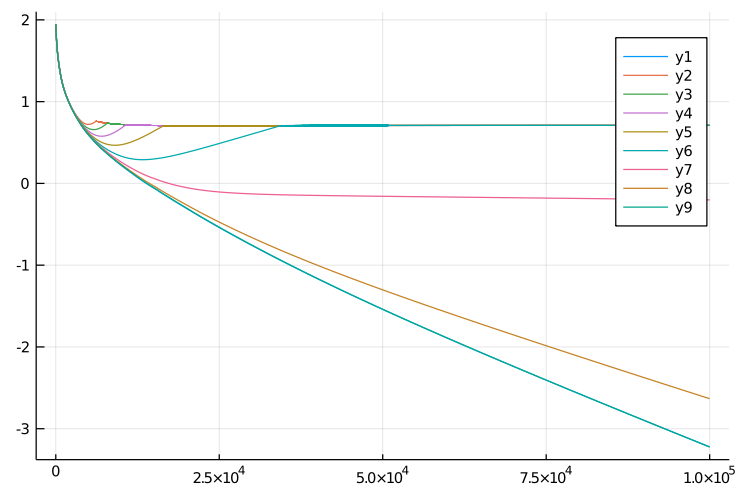
\includegraphics[width=0.80\textwidth]{NesterovParameters}
\caption{$||\partial L||$ Log10-scale objective minimization with varying parameters of the Nesterov Momentum algorithm. Here the parameters are encompassing a relative variation of only $10^{-8}$, but the algorithm dynamic is completely changing}
\label{fig:NesterovParameters}
\end{figure}
\begin{figure}[ht]
\centering
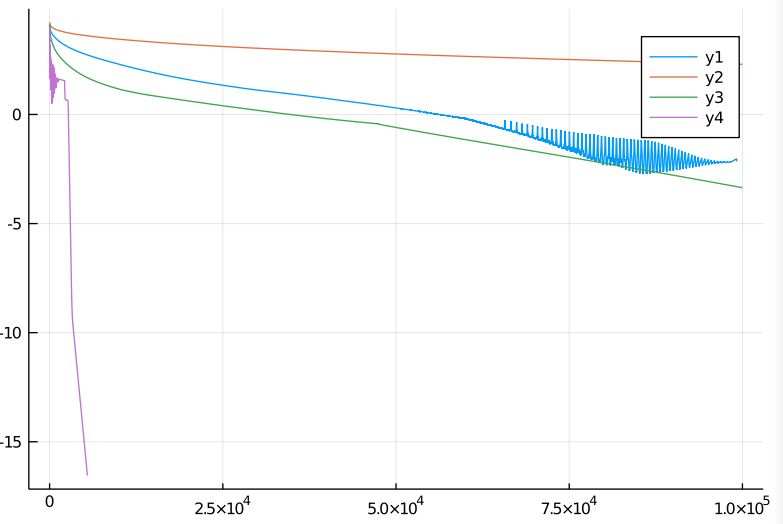
\includegraphics[width=0.80\textwidth]{RMSPropParameters}
\caption{$||\partial L||$ Log10-scale objective minimization with varying parameters of the RMSProp algorithm. Usually, varying the parameters of such algorithms, it is possible to reach a "stationary point" for the dynamics; sometimes, with a stroke of luck, as in this case, moving a bit further may lead to a point where the dynamics is initially less stable, afterward incredibly faster}
\label{fig:RMSPropParameters}
\end{figure}
\begin{figure}[ht]
\centering
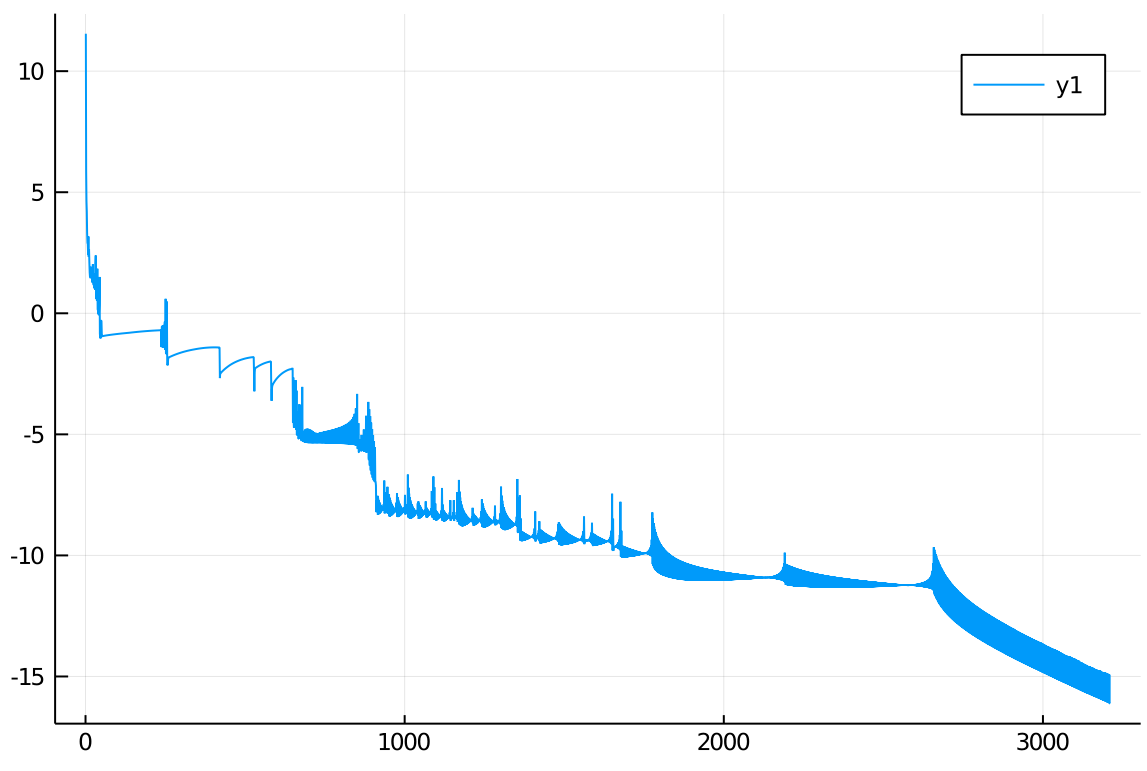
\includegraphics[width=0.80\textwidth]{PCG}
\caption{$||E x - b||^2$ Log10-scale objective minimization typical dynamics of projected conjugate gradient with long search + local search, here on a $1000\times 2000$ incidence matrix $E$.}
\label{fig:PCG}
\end{figure}
\begin{figure}[ht]
\centering
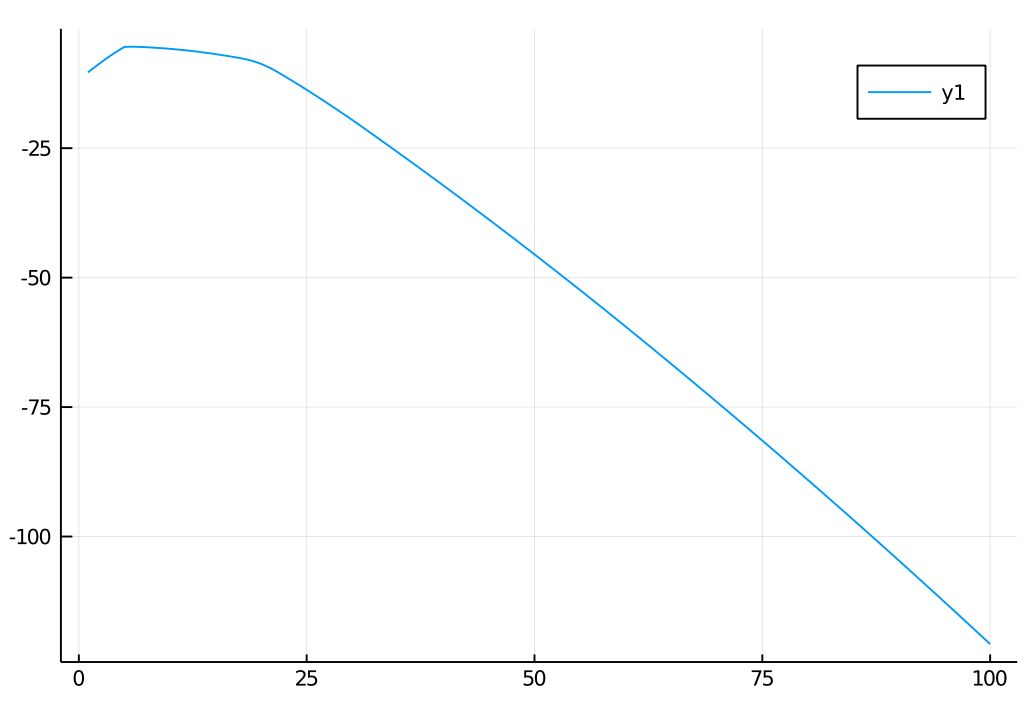
\includegraphics[width=0.80\textwidth]{LineSearch}
\caption{$L(\mu+\alpha d)$ Lagrangian dual (D1) restricted to the direction of line search when $Q$ is singular; here the primal $x$ corresponds to the subgradient we choose on the top vertex.}
\label{fig:LineSearch}
\end{figure}

%\clearpage
%\tableofcontents

\end{document}
